% Options for packages loaded elsewhere
\PassOptionsToPackage{unicode}{hyperref}
\PassOptionsToPackage{hyphens}{url}
%
\documentclass[
]{article}
\title{Informações sobre barragens de mineração}
\author{Márcio Augusto F. Rodrigues}
\date{Agosto de 2022}

\usepackage{amsmath,amssymb}
\usepackage{lmodern}
\usepackage{iftex}
\ifPDFTeX
  \usepackage[T1]{fontenc}
  \usepackage[utf8]{inputenc}
  \usepackage{textcomp} % provide euro and other symbols
\else % if luatex or xetex
  \usepackage{unicode-math}
  \defaultfontfeatures{Scale=MatchLowercase}
  \defaultfontfeatures[\rmfamily]{Ligatures=TeX,Scale=1}
\fi
% Use upquote if available, for straight quotes in verbatim environments
\IfFileExists{upquote.sty}{\usepackage{upquote}}{}
\IfFileExists{microtype.sty}{% use microtype if available
  \usepackage[]{microtype}
  \UseMicrotypeSet[protrusion]{basicmath} % disable protrusion for tt fonts
}{}
\makeatletter
\@ifundefined{KOMAClassName}{% if non-KOMA class
  \IfFileExists{parskip.sty}{%
    \usepackage{parskip}
  }{% else
    \setlength{\parindent}{0pt}
    \setlength{\parskip}{6pt plus 2pt minus 1pt}}
}{% if KOMA class
  \KOMAoptions{parskip=half}}
\makeatother
\usepackage{xcolor}
\IfFileExists{xurl.sty}{\usepackage{xurl}}{} % add URL line breaks if available
\IfFileExists{bookmark.sty}{\usepackage{bookmark}}{\usepackage{hyperref}}
\hypersetup{
  pdftitle={Informações sobre barragens de mineração},
  pdfauthor={Márcio Augusto F. Rodrigues},
  hidelinks,
  pdfcreator={LaTeX via pandoc}}
\urlstyle{same} % disable monospaced font for URLs
\usepackage[margin=1in]{geometry}
\usepackage{color}
\usepackage{fancyvrb}
\newcommand{\VerbBar}{|}
\newcommand{\VERB}{\Verb[commandchars=\\\{\}]}
\DefineVerbatimEnvironment{Highlighting}{Verbatim}{commandchars=\\\{\}}
% Add ',fontsize=\small' for more characters per line
\usepackage{framed}
\definecolor{shadecolor}{RGB}{248,248,248}
\newenvironment{Shaded}{\begin{snugshade}}{\end{snugshade}}
\newcommand{\AlertTok}[1]{\textcolor[rgb]{0.94,0.16,0.16}{#1}}
\newcommand{\AnnotationTok}[1]{\textcolor[rgb]{0.56,0.35,0.01}{\textbf{\textit{#1}}}}
\newcommand{\AttributeTok}[1]{\textcolor[rgb]{0.77,0.63,0.00}{#1}}
\newcommand{\BaseNTok}[1]{\textcolor[rgb]{0.00,0.00,0.81}{#1}}
\newcommand{\BuiltInTok}[1]{#1}
\newcommand{\CharTok}[1]{\textcolor[rgb]{0.31,0.60,0.02}{#1}}
\newcommand{\CommentTok}[1]{\textcolor[rgb]{0.56,0.35,0.01}{\textit{#1}}}
\newcommand{\CommentVarTok}[1]{\textcolor[rgb]{0.56,0.35,0.01}{\textbf{\textit{#1}}}}
\newcommand{\ConstantTok}[1]{\textcolor[rgb]{0.00,0.00,0.00}{#1}}
\newcommand{\ControlFlowTok}[1]{\textcolor[rgb]{0.13,0.29,0.53}{\textbf{#1}}}
\newcommand{\DataTypeTok}[1]{\textcolor[rgb]{0.13,0.29,0.53}{#1}}
\newcommand{\DecValTok}[1]{\textcolor[rgb]{0.00,0.00,0.81}{#1}}
\newcommand{\DocumentationTok}[1]{\textcolor[rgb]{0.56,0.35,0.01}{\textbf{\textit{#1}}}}
\newcommand{\ErrorTok}[1]{\textcolor[rgb]{0.64,0.00,0.00}{\textbf{#1}}}
\newcommand{\ExtensionTok}[1]{#1}
\newcommand{\FloatTok}[1]{\textcolor[rgb]{0.00,0.00,0.81}{#1}}
\newcommand{\FunctionTok}[1]{\textcolor[rgb]{0.00,0.00,0.00}{#1}}
\newcommand{\ImportTok}[1]{#1}
\newcommand{\InformationTok}[1]{\textcolor[rgb]{0.56,0.35,0.01}{\textbf{\textit{#1}}}}
\newcommand{\KeywordTok}[1]{\textcolor[rgb]{0.13,0.29,0.53}{\textbf{#1}}}
\newcommand{\NormalTok}[1]{#1}
\newcommand{\OperatorTok}[1]{\textcolor[rgb]{0.81,0.36,0.00}{\textbf{#1}}}
\newcommand{\OtherTok}[1]{\textcolor[rgb]{0.56,0.35,0.01}{#1}}
\newcommand{\PreprocessorTok}[1]{\textcolor[rgb]{0.56,0.35,0.01}{\textit{#1}}}
\newcommand{\RegionMarkerTok}[1]{#1}
\newcommand{\SpecialCharTok}[1]{\textcolor[rgb]{0.00,0.00,0.00}{#1}}
\newcommand{\SpecialStringTok}[1]{\textcolor[rgb]{0.31,0.60,0.02}{#1}}
\newcommand{\StringTok}[1]{\textcolor[rgb]{0.31,0.60,0.02}{#1}}
\newcommand{\VariableTok}[1]{\textcolor[rgb]{0.00,0.00,0.00}{#1}}
\newcommand{\VerbatimStringTok}[1]{\textcolor[rgb]{0.31,0.60,0.02}{#1}}
\newcommand{\WarningTok}[1]{\textcolor[rgb]{0.56,0.35,0.01}{\textbf{\textit{#1}}}}
\usepackage{longtable,booktabs,array}
\usepackage{calc} % for calculating minipage widths
% Correct order of tables after \paragraph or \subparagraph
\usepackage{etoolbox}
\makeatletter
\patchcmd\longtable{\par}{\if@noskipsec\mbox{}\fi\par}{}{}
\makeatother
% Allow footnotes in longtable head/foot
\IfFileExists{footnotehyper.sty}{\usepackage{footnotehyper}}{\usepackage{footnote}}
\makesavenoteenv{longtable}
\usepackage{graphicx}
\makeatletter
\def\maxwidth{\ifdim\Gin@nat@width>\linewidth\linewidth\else\Gin@nat@width\fi}
\def\maxheight{\ifdim\Gin@nat@height>\textheight\textheight\else\Gin@nat@height\fi}
\makeatother
% Scale images if necessary, so that they will not overflow the page
% margins by default, and it is still possible to overwrite the defaults
% using explicit options in \includegraphics[width, height, ...]{}
\setkeys{Gin}{width=\maxwidth,height=\maxheight,keepaspectratio}
% Set default figure placement to htbp
\makeatletter
\def\fps@figure{htbp}
\makeatother
\setlength{\emergencystretch}{3em} % prevent overfull lines
\providecommand{\tightlist}{%
  \setlength{\itemsep}{0pt}\setlength{\parskip}{0pt}}
\setcounter{secnumdepth}{-\maxdimen} % remove section numbering
\ifLuaTeX
  \usepackage{selnolig}  % disable illegal ligatures
\fi

\begin{document}
\maketitle

\hypertarget{objetivos}{%
\subsection{Objetivos}\label{objetivos}}

Este relatório tem como objetivo apresentar funcionalidades do \emph{R
Markdown} e do \emph{Quarto}, utilizando dados públicos sobre barragens
de mineração no Brasil.

Os objetivos específicos da análise são:

\begin{itemize}
\tightlist
\item
  fazer uma tabela das barragens por estado;
\item
  fazer um gráfico do número de barragens por categoria de dano
  potencial associado;
\end{itemize}

\hypertarget{materiais-e-muxe9todos}{%
\subsection{Materiais e métodos}\label{materiais-e-muxe9todos}}

A base de dados disponibilizada pelo
\href{https://app.anm.gov.br/SIGBM/Publico/ClassificacaoNacionalDaBarragem}{SIGBM
- Sistema de Gestão de Segurança de Barragem de Mineração} apresenta
dados referentes à Barragens de Mineração no território brasileiro.

\hypertarget{carregando-os-pacotes}{%
\subsection{Carregando os pacotes}\label{carregando-os-pacotes}}

\begin{Shaded}
\begin{Highlighting}[]
\FunctionTok{library}\NormalTok{(gt)}
\FunctionTok{library}\NormalTok{(janitor)}
\FunctionTok{library}\NormalTok{(tidyverse)}
\FunctionTok{library}\NormalTok{(readxl)}
\end{Highlighting}
\end{Shaded}

\hypertarget{download-e-leitura-da-base}{%
\subsection{Download e leitura da
base}\label{download-e-leitura-da-base}}

\hypertarget{download}{%
\subsubsection{Download}\label{download}}

\hypertarget{leitura}{%
\subsubsection{Leitura}\label{leitura}}

\begin{Shaded}
\begin{Highlighting}[]
\CommentTok{\# Importar a base de dados:}
\CommentTok{\# ler os dados baixados}
\NormalTok{sigbm }\OtherTok{\textless{}{-}} \FunctionTok{read\_xlsx}\NormalTok{(}\StringTok{"dados/sigbm.xlsx"}\NormalTok{, }\AttributeTok{skip =} \DecValTok{4}\NormalTok{) }\SpecialCharTok{|}\ErrorTok{\textgreater{}}
  \FunctionTok{clean\_names}\NormalTok{()}
\end{Highlighting}
\end{Shaded}

Data de atualização da base

\begin{Shaded}
\begin{Highlighting}[]
\CommentTok{\# {-}{-}{-}{-}{-} data de atualização {-}{-}{-}{-}{-}}
\NormalTok{data\_atualizacao\_sigbm }\OtherTok{\textless{}{-}} \FunctionTok{read\_xlsx}\NormalTok{(}\StringTok{"dados/sigbm.xlsx"}\NormalTok{,}
                                    \AttributeTok{col\_names =} \ConstantTok{FALSE}\NormalTok{,}
                                    \AttributeTok{n\_max =} \DecValTok{1}\NormalTok{) }\SpecialCharTok{|}\ErrorTok{\textgreater{}}
  \FunctionTok{pull}\NormalTok{() }\SpecialCharTok{|}\ErrorTok{\textgreater{}}
  \FunctionTok{str\_extract}\NormalTok{(}\StringTok{":.*{-}"}\NormalTok{) }\SpecialCharTok{|}\ErrorTok{\textgreater{}}
  \FunctionTok{str\_remove}\NormalTok{(}\StringTok{":"}\NormalTok{) }\SpecialCharTok{|}\ErrorTok{\textgreater{}}
  \FunctionTok{str\_remove}\NormalTok{(}\StringTok{"{-}"}\NormalTok{) }\SpecialCharTok{|}\ErrorTok{\textgreater{}}
  \FunctionTok{str\_trim}\NormalTok{()}
\end{Highlighting}
\end{Shaded}

\hypertarget{barragens-de-minerauxe7uxe3o-no-brasil}{%
\subsection{Barragens de mineração no
Brasil}\label{barragens-de-minerauxe7uxe3o-no-brasil}}

A base do SIGBM foi obtida no dia 16/08/2022, e apresentou informações
referentes a 911.

\hypertarget{tabela}{%
\subsection{Tabela}\label{tabela}}

\begin{Shaded}
\begin{Highlighting}[]
\NormalTok{sigbm }\SpecialCharTok{|}\ErrorTok{\textgreater{}}
  \FunctionTok{count}\NormalTok{(uf, }\AttributeTok{sort =} \ConstantTok{TRUE}\NormalTok{) }\SpecialCharTok{|}\ErrorTok{\textgreater{}}
  \FunctionTok{slice}\NormalTok{(}\DecValTok{1}\SpecialCharTok{:}\DecValTok{10}\NormalTok{) }\SpecialCharTok{|}\ErrorTok{\textgreater{}}
  \FunctionTok{select}\NormalTok{(}\StringTok{\textasciigrave{}}\AttributeTok{Estado}\StringTok{\textasciigrave{}} \OtherTok{=}\NormalTok{ uf, }\StringTok{\textasciigrave{}}\AttributeTok{Número de barragens}\StringTok{\textasciigrave{}} \OtherTok{=}\NormalTok{ n) }\SpecialCharTok{|}\ErrorTok{\textgreater{}}
  \CommentTok{\#gt::gt(caption = "Dez estados brasileiros com mais barragens cadastradas no SIG{-}BM") \#\# para pdf e html}
\NormalTok{  knitr}\SpecialCharTok{::}\FunctionTok{kable}\NormalTok{(}\AttributeTok{caption =} \StringTok{"Dez estados brasileiros com mais barragens cadastradas no SIG{-}BM"}\NormalTok{) }\CommentTok{\# para criar tabelas em word}
\end{Highlighting}
\end{Shaded}

\begin{longtable}[]{@{}lr@{}}
\caption{Dez estados brasileiros com mais barragens cadastradas no
SIG-BM}\tabularnewline
\toprule
Estado & Número de barragens \\
\midrule
\endfirsthead
\toprule
Estado & Número de barragens \\
\midrule
\endhead
MG & 346 \\
MT & 152 \\
PA & 114 \\
BA & 82 \\
SP & 68 \\
RO & 36 \\
GO & 22 \\
AP & 18 \\
MS & 18 \\
AM & 15 \\
\bottomrule
\end{longtable}

\hypertarget{gruxe1fico}{%
\subsection{Gráfico}\label{gruxe1fico}}

\begin{Shaded}
\begin{Highlighting}[]
\DocumentationTok{\#\# {-}{-}{-}{-}plot{-}dpa{-}{-}{-}{-}{-}{-}{-}{-}{-}{-}{-}{-}{-}{-}{-}{-}{-}{-}{-}{-}{-}{-}{-}{-}{-}{-}{-}}
\NormalTok{sigbm }\SpecialCharTok{|}\ErrorTok{\textgreater{}}
  \FunctionTok{count}\NormalTok{(dano\_potencial\_associado) }\SpecialCharTok{|}\ErrorTok{\textgreater{}}
    \FunctionTok{mutate}\NormalTok{(}
    \AttributeTok{dano\_potencial\_associado =} \FunctionTok{if\_else}\NormalTok{(}
\NormalTok{      dano\_potencial\_associado }\SpecialCharTok{==} \StringTok{"N/A"}\NormalTok{,}
      \StringTok{"Não se aplica"}\NormalTok{,}
\NormalTok{      dano\_potencial\_associado}
\NormalTok{    ),}
    \AttributeTok{dano\_potencial\_associado =} \FunctionTok{factor}\NormalTok{(}
\NormalTok{      dano\_potencial\_associado,}
      \AttributeTok{levels =} \FunctionTok{c}\NormalTok{(}\StringTok{"Não se aplica"}\NormalTok{, }\StringTok{"Baixo"}\NormalTok{, }\StringTok{"Médio"}\NormalTok{, }\StringTok{"Alto"}\NormalTok{)}
\NormalTok{    )}
\NormalTok{  ) }\SpecialCharTok{|}\ErrorTok{\textgreater{}}
  \FunctionTok{ggplot}\NormalTok{() }\SpecialCharTok{+}
  \FunctionTok{aes}\NormalTok{(}\AttributeTok{x =}\NormalTok{ dano\_potencial\_associado, }\AttributeTok{y =}\NormalTok{ n) }\SpecialCharTok{+}
  \FunctionTok{geom\_col}\NormalTok{(}\AttributeTok{fill =} \StringTok{"lightblue"}\NormalTok{) }\SpecialCharTok{+}
  \FunctionTok{theme\_bw}\NormalTok{() }\SpecialCharTok{+}
  \FunctionTok{labs}\NormalTok{(}\AttributeTok{x =} \StringTok{"Dano potencial associado (DPA)"}\NormalTok{, }\AttributeTok{y =} \StringTok{"Quantidade de barragens"}\NormalTok{,}
       \AttributeTok{title =} \StringTok{"Dano potencial associado de barragens de mineração no Brasil"}\NormalTok{)}
\end{Highlighting}
\end{Shaded}

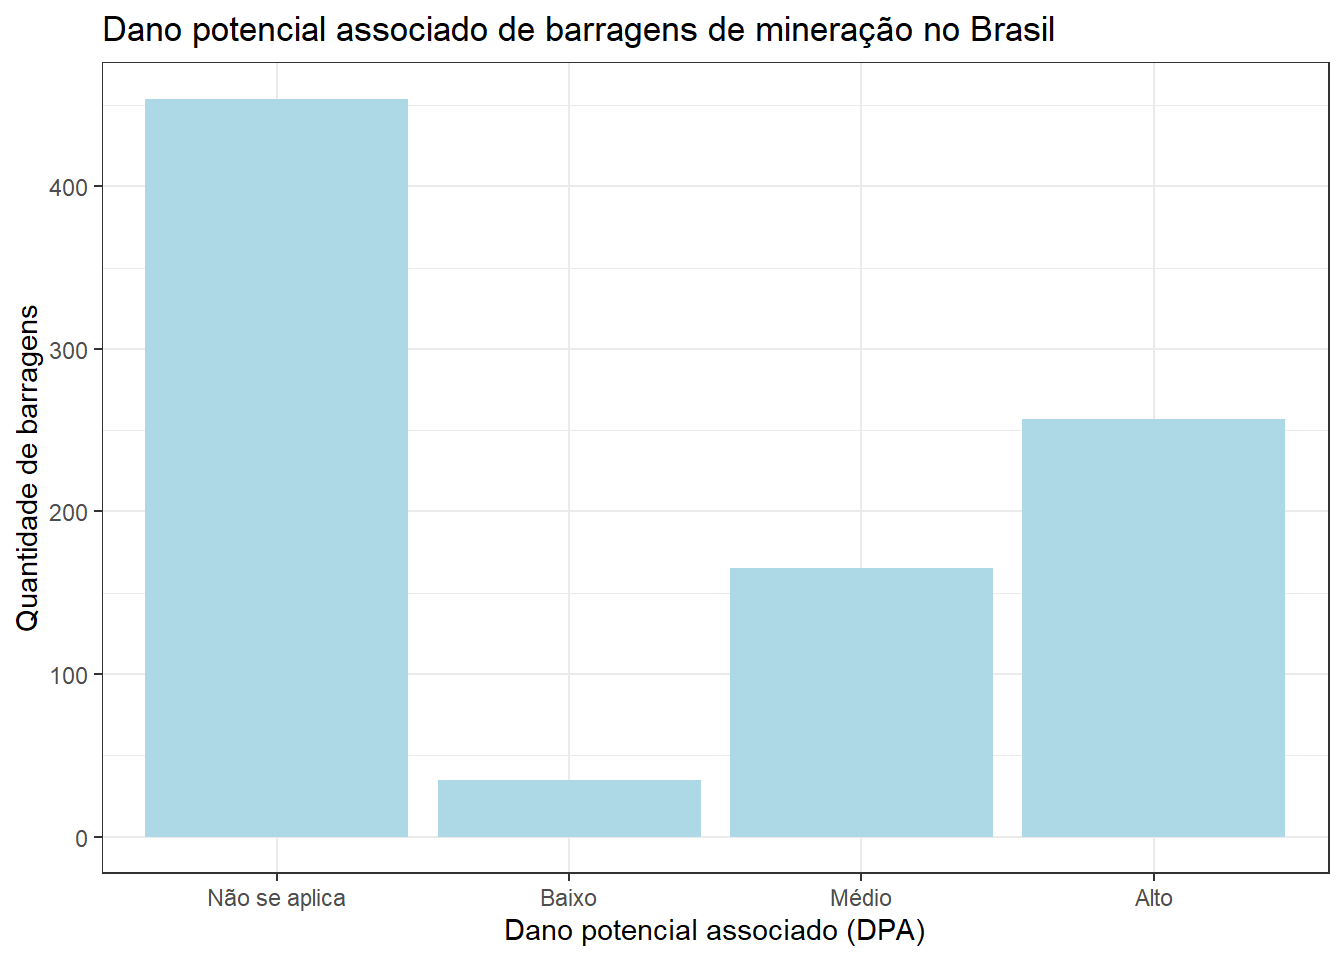
\includegraphics{pratica1_files/figure-latex/unnamed-chunk-6-1.pdf}

\end{document}
